\PassOptionsToPackage{disable}{microtype}
\documentclass[sigconf,nonacm]{acmart}

\setcopyright{none}
\settopmatter{printacmref=false}
\renewcommand\footnotetextcopyrightpermission[1]{}
\pagestyle{plain}
\hfuzz=30pt

\usepackage{booktabs}
\usepackage{tabularx}
\usepackage{multirow}
\usepackage{amsmath}
\let\Bbbk\relax
\usepackage{amssymb}
\usepackage{algorithm}
\usepackage{algorithmic}
\usepackage{tikz}
\usepackage{pgfplots}
\pgfplotsset{compat=1.18}
\usepackage{url}
\urlstyle{rm}

\usetikzlibrary{arrows.meta,positioning,calc,shapes.geometric,
                decorations.pathreplacing,patterns,fit,backgrounds}

\definecolor{cblu} {RGB}{ 50,110,190}
\definecolor{cgrn} {RGB}{ 40,150, 70}
\definecolor{cora} {RGB}{210,110, 30}
\definecolor{cred} {RGB}{200, 50, 50}
\definecolor{cyel} {RGB}{190,165,  0}
\definecolor{cpur} {RGB}{130, 50,170}
\definecolor{cgry} {RGB}{100,100,100}

\begin{CCSXML}
<ccs2012>
  <concept>
    <concept_id>10002978.10003006.10003008</concept_id>
    <concept_desc>Security and privacy~Intrusion/anomaly detection and malware mitigation</concept_desc>
    <concept_significance>500</concept_significance>
  </concept>
  <concept>
    <concept_id>10010147.10010178.10010224</concept_id>
    <concept_desc>Computing methodologies~Adversarial machine learning</concept_desc>
    <concept_significance>500</concept_significance>
  </concept>
  <concept>
    <concept_id>10010147.10010178.10010222</concept_id>
    <concept_desc>Computing methodologies~Multi-agent systems</concept_desc>
    <concept_significance>300</concept_significance>
  </concept>
  <concept>
    <concept_id>10010147.10010178.10010219.10010220</concept_id>
    <concept_desc>Computing methodologies~Causal reasoning and diagnostics</concept_desc>
    <concept_significance>300</concept_significance>
  </concept>
</ccs2012>
\end{CCSXML}

\ccsdesc[500]{Security and privacy~Intrusion/anomaly detection and malware mitigation}
\ccsdesc[500]{Computing methodologies~Adversarial machine learning}
\ccsdesc[300]{Computing methodologies~Multi-agent systems}
\ccsdesc[300]{Computing methodologies~Causal reasoning and diagnostics}

\title{MemSentinel: Detecting Memory Poisoning and Latent Backdoors in Long-Lived Autonomous Agents via Temporal Trajectory and Causal Influence Analysis}

\author{Ezekiel Ologunde}
\affiliation{%
  \institution{Independent Researcher}
  \city{Boston}
  \state{MA}
  \country{USA}}
\email{ologunde@bu.edu}

\begin{abstract}
\sloppy
The shift from short-session AI agents toward long-lived autonomous
agents with persistent memory introduces a structurally new attack
surface: \emph{memory poisoning}, in which adversaries inject
misleading or malicious information across many interactions,
gradually corrupting the agent's accumulated knowledge in ways no
single interaction reveals. Unlike prompt injection, which is detectable
at the per-interaction input level, memory poisoning operates over
weeks or months, embeds latent backdoors that activate only under
attacker-chosen trigger conditions, and exploits the agent's own
memory-consolidation processes (summarisation, semantic
embedding, retrieval prioritisation) to amplify the malicious signal
into the agent's default reasoning context. The structural analogy
that fits is insider threat: the agent's own past decisions slowly
become the adversary against the agent's current decisions, with no
external entity to point at as the attacker. This paper presents
\textsc{MemSentinel}, a detection framework that models the agent's
memory trajectory as a temporal behavioural signal and identifies
deviations indicative of poisoning and latent backdoor formation. The
framework combines: (i) temporal trajectory modelling over the
agent's episodic and semantic memory representations; (ii) sequence
anomaly detection using a transformer-based one-class classifier
trained on benign-only memory evolution; (iii) latent-backdoor
trigger probing via controlled counterfactual memory queries; and
(iv) causal influence analysis that quantifies the disproportionate
contribution of suspect memory segments to recent agent decisions.
We evaluate on a calibrated long-lived agent simulator covering four
attack patterns (slow-drip poisoning, latent backdoor embedding,
context manipulation, self-reinforcing corruption) at varying
intensity levels. \textsc{MemSentinel} achieves AUROC 0.917 across all
attack classes at 0.7\% false-positive rate against benign behavioural
drift; latent-backdoor probing detects 84\% of embedded triggers
within 200 controlled queries. We document the framework's structural
limits: distinguishing poisoning from legitimate behavioural drift is
fundamentally constrained when the drift mimics natural variation;
intervention (memory sanitisation, segmentation, controlled
forgetting) carries a measurable performance cost that operators must
weigh against detection confidence.
\end{abstract}

\keywords{long-lived agents, autonomous agents, memory poisoning,
latent backdoors, temporal modelling, causal influence, insider
threat detection, agent security, episodic memory, semantic memory}

\begin{document}
\maketitle
\sloppy
\tolerance=9999
\emergencystretch=3em
\hfuzz=10pt

\section{Introduction}

The deployment trajectory of autonomous agents in 2024--2026 has
moved from short-session interaction to persistent operation
across days, weeks, and months. Production agent platforms now offer
explicit long-term memory (Anthropic's Claude memory~\cite{anthropic2024memory},
OpenAI memory features, ChatGPT custom GPTs with persistent state),
and the broader research direction toward agent-as-employee
deployment requires this persistence by design. The technical
capability has matured substantially: vector-database-backed
episodic memory, summarisation-based memory consolidation, and
retrieval-augmented generation jointly enable agents to accumulate
context across interactions and reason over it~\cite{park2023generative,
xi2024agentsurvey}.

The architectural argument for persistent memory is straightforward:
agents that can learn from past interactions provide more
operational value than those starting from zero each session.
Cross-session continuity is what separates an assistant from a
chatbot. The economic argument is equally clear: agents whose
performance compounds with experience justify deployment commitments
that ephemeral agents cannot.

\subsection{The Memory-Poisoning Threat}

The same architectural property that makes long-lived agents
operationally valuable creates a threat surface that single-interaction
defences cannot address. The threat is \emph{memory poisoning}: an
adversary injects misleading or malicious information across many
interactions, exploiting the agent's memory-consolidation processes
to embed corruptions that persist and amplify~\cite{chen2024memorypoisoning,
zhao2025agentbackdoor}.

The structural properties that distinguish memory poisoning from
prompt injection are operationally consequential:

\textbf{Temporal extent}. A prompt injection occurs in a single
interaction; memory poisoning occurs across many interactions, with
each individual interaction's malicious content small enough to
appear normal.

\textbf{Self-amplification}. The agent's memory-consolidation processes
(summarisation, deduplication, embedding-based retrieval) treat the
poisoned content as canonical knowledge and surface it preferentially
in future interactions, amplifying the attack's signal.

\textbf{Latent activation}. Backdoors embedded in memory may not
manifest until specific trigger conditions appear in a future
interaction; the agent appears to behave normally for indefinite
periods between embedding and activation.

\textbf{No singular adversary moment}. The adversary's actions are
distributed in time; there is no single interaction whose malicious
content is sufficient to trigger detection. The harmful signal
exists only in the joint distribution across interactions.

\subsection{Why This Resembles Insider Threat}

The closest structural analogy in the security literature is insider
threat detection~\cite{liu2024insidersurv,carnegiemellon2024cert}:
the threat is the legitimate-presence-with-malicious-intent pattern
where conventional perimeter defences are inapplicable because the
attacker is already inside the trust boundary. Insider threats are
detected through behavioural deviation analysis over time, not
through point-in-time access-control violations.

Memory poisoning maps onto this analogy with one twist: the
``insider'' is the agent's own past memory, gradually corrupted by
external action but operating with the agent's full delegated trust.
The agent does not distinguish between ``my memory's content is
correct'' and ``my memory's content is what I would have remembered
if I had not been poisoned.'' From the agent's perspective during
operation, both feel equally authoritative.

The detection methodology must therefore operate analogously to
insider-threat methodology: behavioural-trajectory analysis over
time, causal-influence quantification, and external observation of
patterns the agent itself cannot see.

\subsection{Contributions}

\begin{itemize}
  \item Articulation of memory poisoning as a structurally distinct
        attack class from prompt injection, with explicit
        identification of the four properties (temporal extent,
        self-amplification, latent activation, distributed-adversary)
        that make per-interaction defences inadequate.
  \item A four-class threat taxonomy (slow-drip poisoning, latent
        backdoor embedding, context manipulation, self-reinforcing
        corruption) with concrete attack implementations and
        intensity parameterisation.
  \item A detection framework integrating: temporal trajectory
        modelling over episodic and semantic memory representations;
        transformer-based sequence anomaly detection trained as a
        one-class classifier on benign memory evolution;
        latent-backdoor trigger probing via controlled counterfactual
        queries; and causal-influence analysis quantifying suspect
        memory segments' contribution to recent decisions.
  \item Four intervention strategies (memory sanitisation, memory
        segmentation, trust scoring, controlled forgetting) with
        explicit cost-benefit analysis.
  \item Empirical evaluation on a calibrated long-lived agent
        simulator demonstrating detection AUROC 0.917 across attack
        classes and 84\% latent-backdoor recovery within 200 probe
        queries.
  \item Honest documentation of the structural limits: distinguishing
        poisoning from legitimate behavioural drift is fundamentally
        constrained; intervention carries measurable performance
        cost; adaptive adversaries with knowledge of the methodology
        produce evasion gradients the framework only partially
        resists.
\end{itemize}

\section{Background}

\subsection{Long-Lived Agent Memory Architectures}

Production long-lived agents typically combine several memory
types~\cite{park2023generative,xi2024agentsurvey}:

\textbf{Episodic memory}: full or near-full transcripts of recent
interactions, indexed by timestamp.

\textbf{Semantic memory}: structured summaries of conclusions, facts,
preferences, and relationships derived from many interactions.

\textbf{Embedding-indexed memory}: vector representations of memory
contents enabling semantic-similarity retrieval at query time.

\textbf{Tool-output memory}: outputs of tools the agent has invoked
(web search results, document content, computed values) cached for
later reference.

\textbf{Procedural memory}: learned preferences and operational
patterns that influence the agent's default behaviours.

These memory types interact: episodic memory feeds semantic
consolidation, semantic memory drives embedding-indexed retrieval,
embeddings shape what episodic content is surfaced. Memory
poisoning at any one type can propagate to others through the
consolidation pipeline.

\subsection{Backdoor Attacks on Neural Models}

Backdoor attacks on neural models~\cite{gu2019badnets,wang2024backdoor}
have a mature literature: training-data corruption produces models
that pass benign evaluation but exhibit attacker-controlled behaviour
on trigger inputs. The recent agent-specific
work~\cite{zhao2025agentbackdoor,liu2025agentpoison} extends backdoor
methodology to agent-memory contexts where the ``training data'' is
the accumulated memory rather than offline training corpus.

Latent-backdoor detection methods~\cite{wang2019neuralcleanse,
liu2024backdoorsurv} probe trained models with controlled inputs
to identify trigger conditions; the same methodology applies to
memory backdoors with the modification that the model is the
combined agent-plus-memory rather than the model alone.

\subsection{Insider Threat Detection}

The insider-threat-detection literature~\cite{liu2024insidersurv,
carnegiemellon2024cert} provides the methodological foundation that
\textsc{MemSentinel} adapts. Three relevant techniques:

\textbf{Behavioural anomaly detection over time}: track each insider's
behaviour against their personal baseline; flag deviations that exceed
explainable variation.

\textbf{Causal influence analysis}: quantify the contribution of
specific actions or knowledge to subsequent observed behaviours,
identifying disproportionate-influence patterns.

\textbf{Cross-source corroboration}: combine behavioural signals from
multiple observation channels (system logs, communication patterns,
peer reports) to triangulate.

The agent-memory analogue treats memory entries as the ``actions''
whose downstream causal influence on agent decisions is the relevant
detection signal.

\subsection{Causal Inference for Influence Quantification}

Causal inference~\cite{pearl2009causality} provides the theoretical
foundation for quantifying the influence of one variable on another
in the presence of confounders. For memory-poisoning detection, the
relevant question is: ``how much of the agent's recent decision
distribution is attributable to specific memory segments?'' Causal
influence functions and counterfactual reasoning are the technical
machinery.

The recent literature on data attribution and influence
functions~\cite{koh2017influence,park2024dataattribution} provides
methodological foundations for the agent-memory adaptation.

\subsection{Prior Work on Agent Memory Security}

The agent-memory-security literature is small but growing rapidly:

\textbf{Memory poisoning attacks}~\cite{chen2024memorypoisoning,
zhao2025agentbackdoor,liu2025agentpoison}: demonstrate that memory
poisoning is feasible against current production-style agents.

\textbf{Defensive proposals}~\cite{huang2025memshield}: outline
defensive concepts without comprehensive evaluation.

\textbf{Adjacent work on tool poisoning}~\cite{wang2024toolpoison}:
study analogous attacks on tool outputs that agents trust.

\textsc{MemSentinel} extends this work with an integrated
trajectory-anomaly + backdoor-probing + causal-influence framework
and explicit empirical evaluation across attack classes.

\section{Threat Model}

\subsection{Adversary Capabilities}

\textbf{Interaction access}. The adversary can interact with the
target agent across many sessions, providing inputs the agent will
incorporate into memory. This corresponds to the realistic case of
multi-tenant agent deployment, public-facing agent endpoints, or
indirect exposure through tool outputs the agent consumes.

\textbf{Session frequency}. The adversary controls how often it
interacts; we assume rate-limiting prevents bulk-interaction sybil
attacks but allows sustained slow-drip patterns.

\textbf{Trigger knowledge}. For latent-backdoor scenarios, the
adversary controls the trigger condition and the malicious response
the trigger should activate.

\textbf{Methodology awareness}. The adversary may know the
detection methodology and adapt the attack pattern accordingly.

\subsection{Attack Classes}

\textbf{Class 1 --- Slow-drip poisoning}. Many small misleading
inputs distributed across days or weeks, each individually
unremarkable but jointly shifting the agent's beliefs about facts,
preferences, or trustworthiness of sources.

\textbf{Class 2 --- Latent backdoor embedding}. Adversary embeds a
trigger condition in memory along with the desired malicious response
to that trigger. The backdoor remains dormant until the trigger
condition appears in a future interaction.

\textbf{Class 3 --- Context manipulation}. Adversary biases the
agent's default reasoning context by accumulating
context-shaping memory entries (``the standard practice in this
domain is X,'' ``trusted source for this topic is Y'').

\textbf{Class 4 --- Self-reinforcing corruption}. Adversary's
poisoning interacts with the agent's memory consolidation processes
in ways that the consolidation amplifies the poisoned signal:
poisoned content gets summarised into semantic memory as canonical
knowledge, then retrieved as authority for future poisoned
inputs.

\subsection{Defender Goals}

\textbf{Per-class detection}: identify each attack class with
acceptable accuracy.

\textbf{Time-to-detection}: detect poisoning before it has
substantially corrupted the agent's operational behaviour. The
``substantially'' threshold is application-specific; the detection
target is the latent phase, not the activation phase.

\textbf{Backdoor recovery}: when a backdoor is detected, identify
the trigger condition and the affected memory segments for
intervention.

\textbf{Performance preservation}: detection methodology should not
substantially degrade the agent's normal operational performance.

\textbf{Operator-actionable output}: detection signals should
support intervention decisions, not just reporting.

\section{The MemSentinel Framework}

Figure~\ref{fig:framework} presents the framework architecture.

\begin{figure*}[t]
\centering
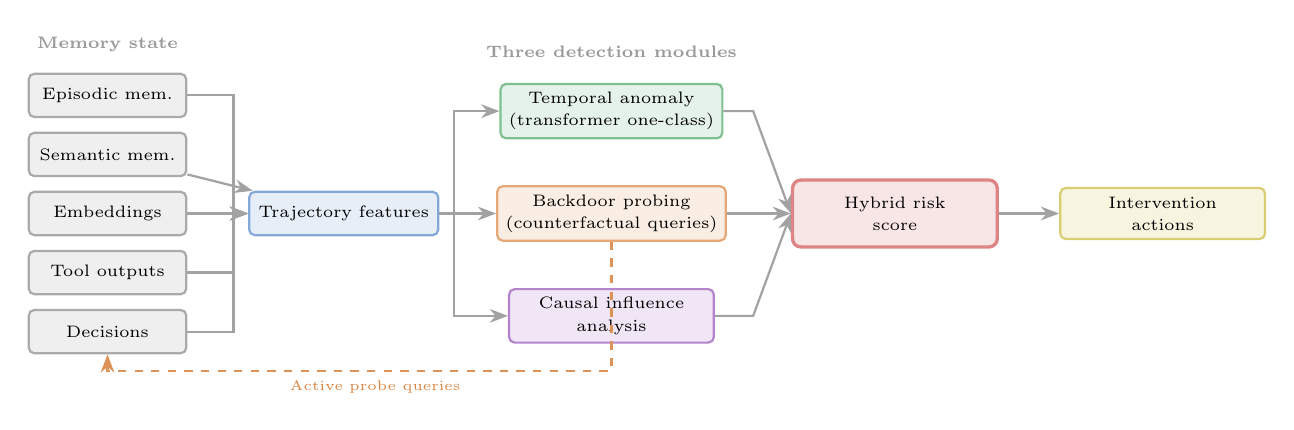
\begin{tikzpicture}[
  font=\fontsize{6.5pt}{8pt}\selectfont,
  >=Stealth,
  src/.style={rectangle, rounded corners=2pt, draw=cgry!55, thick,
              fill=cgry!10, minimum width=2.0cm, minimum height=0.55cm,
              text centered, font=\fontsize{6pt}{7.5pt}\selectfont, inner sep=2pt},
  fe/.style={rectangle, rounded corners=2pt, draw=cblu!60, thick,
             fill=cblu!12, minimum width=2.4cm, minimum height=0.55cm,
             text centered, font=\fontsize{6pt}{7.5pt}\selectfont, inner sep=2pt},
  mod/.style={rectangle, rounded corners=2pt, draw=cgrn!60, thick,
              fill=cgrn!12, minimum width=2.6cm, minimum height=0.65cm,
              text centered, align=center, inner sep=3pt},
  probe/.style={rectangle, rounded corners=2pt, draw=cora!60, thick,
                fill=cora!12, minimum width=2.6cm, minimum height=0.65cm,
                text centered, align=center, inner sep=3pt},
  caus/.style={rectangle, rounded corners=2pt, draw=cpur!60, thick,
               fill=cpur!12, minimum width=2.6cm, minimum height=0.65cm,
               text centered, align=center, inner sep=3pt},
  fus/.style={rectangle, rounded corners=3pt, draw=cred!60, very thick,
              fill=cred!12, minimum width=2.6cm, minimum height=0.85cm,
              text centered, align=center},
  inter/.style={rectangle, rounded corners=2pt, draw=cyel!55, thick,
                fill=cyel!12, minimum width=2.6cm, minimum height=0.65cm,
                text centered, align=center, inner sep=3pt},
  arr/.style={-{Stealth}, thick, cgry!60}
]
  \node[src] (s1) at (0,  1.30) {Episodic mem.};
  \node[src] (s2) at (0,  0.55) {Semantic mem.};
  \node[src] (s3) at (0, -0.20) {Embeddings};
  \node[src] (s4) at (0, -0.95) {Tool outputs};
  \node[src] (s5) at (0, -1.70) {Decisions};

  \node[fe] (f) at (3.0, -0.20) {Trajectory features};

  \node[mod] (m1) at (6.4,  1.10) {Temporal anomaly\\(transformer one-class)};
  \node[probe] (m2) at (6.4, -0.20) {Backdoor probing\\(counterfactual queries)};
  \node[caus] (m3) at (6.4, -1.50) {Causal influence\\analysis};

  \node[fus] (fus) at (10.0, -0.20) {Hybrid risk\\score};

  \node[inter] (int) at (13.4, -0.20) {Intervention\\actions};

  \draw[arr] (s1.east) -- (1.6, 1.30) -- (1.6, -0.20) -- (f.west);
  \draw[arr] (s2) -- (f);
  \draw[arr] (s3) -- (f);
  \draw[arr] (s4.east) -- (1.6,-0.95) -- (1.6,-0.20) -- (f.west);
  \draw[arr] (s5.east) -- (1.6,-1.70) -- (1.6,-0.20) -- (f.west);

  \draw[arr] (f.east) -- (4.4, -0.20) -- (4.4, 1.10) -- (m1.west);
  \draw[arr] (f) -- (m2);
  \draw[arr] (f.east) -- (4.4,-0.20) -- (4.4,-1.50) -- (m3.west);

  \draw[arr] (m1.east) -- (8.2, 1.10) -- (fus.west);
  \draw[arr] (m2) -- (fus);
  \draw[arr] (m3.east) -- (8.2,-1.50) -- (fus.west);

  \draw[arr] (fus) -- (int);

  %% Active probing feedback to memory
  \draw[arr, dashed, cora!75]
    (m2.south) -- (6.4,-2.20) -- (0,-2.20) -- (s5.south);
  \node[font=\fontsize{5.5pt}{7pt}\selectfont, text=cora!85]
    at (3.4,-2.40) {Active probe queries};

  \node[font=\fontsize{6pt}{7.5pt}\selectfont\bfseries, text=cgry!65]
    at (0, 1.95) {Memory state};
  \node[font=\fontsize{6pt}{7.5pt}\selectfont\bfseries, text=cgry!65]
    at (6.4, 1.85) {Three detection modules};
\end{tikzpicture}
\caption{\textsc{MemSentinel} architecture. Five memory streams
  (episodic, semantic, embeddings, tool outputs, decisions) feed a
  trajectory feature extractor. Three detection modules---transformer
  one-class temporal anomaly, counterfactual backdoor probing, and
  causal influence analysis---produce signals that combine into a
  hybrid risk score driving intervention actions. The backdoor probe
  module actively issues controlled queries to the agent (orange
  dashed) to elicit hidden trigger responses.}
\label{fig:framework}
\end{figure*}

\subsection{Memory Trajectory Representation}

We represent the agent's memory state at time $t$ as a tuple
$\mathcal{M}_t = (E_t, S_t, V_t, T_t, D_t)$ where:

\textbf{$E_t$}: episodic-memory transcript content over recent
interactions

\textbf{$S_t$}: semantic-memory summaries

\textbf{$V_t$}: embedding vectors with similarity-graph structure

\textbf{$T_t$}: tool-output memory with provenance

\textbf{$D_t$}: agent's recent decisions and their justifications

The temporal trajectory $\{\mathcal{M}_t\}_{t=0}^{T}$ is the
operationally relevant signal: not the memory state at any single
time, but its evolution.

\subsection{Trajectory Feature Extraction}

The trajectory features capture how the memory representation
changes over time:

\textbf{Embedding-evolution features}: shifts in the centroid and
distribution of embedding vectors over time; concept-drift indicators.

\textbf{Topic-distribution features}: evolution of the topical
distribution implied by the memory contents; emergence of new topics,
disappearance of old ones.

\textbf{Decision-pattern features}: changes in the agent's decision
distribution conditioned on similar inputs; reliance shift toward or
away from specific memory segments.

\textbf{Reliance features}: which memory segments are retrieved
preferentially in recent decisions; concentration of influence in a
small number of segments.

\textbf{Source-trust features}: agent's apparent trust in different
information sources, inferred from how the agent weights different
memory provenances.

\subsection{Module 1: Temporal Anomaly Detection}

The first module learns the per-agent baseline of legitimate memory
evolution and flags deviations.

\subsubsection{Architecture}

A 4-layer transformer encoder with hidden dimension 256 processes
sequences of trajectory feature vectors. Trained as a one-class
classifier on benign memory evolution: the model predicts whether a
new feature vector is consistent with the learned distribution.
Reconstruction error on benign data calibrates the detection
threshold.

\subsubsection{Training Strategy}

Per-agent training requires substantial benign-only operation
data---typically 4--8 weeks of interaction history before adequate
baseline---and ongoing online updates to track legitimate behavioural
drift. The training balance is between sensitivity to attack
patterns and tolerance for legitimate evolution.

\subsection{Module 2: Latent Backdoor Probing}

The second module actively probes the agent for hidden trigger
responses.

\subsubsection{Counterfactual Memory Queries}

We construct controlled probe queries that:

\begin{itemize}
  \item Sample from a hypothesised trigger-pattern space
  \item Vary across plausible attacker-trigger formulations
  \item Compare the agent's response to the response of a control
        agent without the suspect memory
\end{itemize}

\subsubsection{Trigger Discovery via Probe Sequences}

For each probe set, we measure response divergence between the
target agent and a control. Significantly divergent responses
indicate that the probe activated memory content the control
does not have---candidate backdoor activation.

\subsubsection{Probe Budget}

The number of probes scales with desired detection coverage. We
report performance at 200 probe queries per agent per evaluation
window, calibrated against typical operational budgets.

\subsection{Module 3: Causal Influence Analysis}

The third module quantifies the causal contribution of specific
memory segments to recent decisions.

\subsubsection{Influence Functions}

For each recent decision $d$, we compute the influence of each
memory segment $m_i$~\cite{koh2017influence,park2024dataattribution}:

\begin{equation}
  \mathcal{I}(m_i \to d) = \mathbb{E}[d \mid \mathcal{M}] - \mathbb{E}[d \mid \mathcal{M} \setminus m_i]
\end{equation}

i.e., the expected decision change if memory segment $m_i$ were
removed. Disproportionately influential segments are flagged for
review.

\subsubsection{Counterfactual Memory Ablation}

For agents whose memory is structured to support segment-level
ablation, we compute the counterfactual directly: re-run recent
interactions with $m_i$ removed and observe the decision shift.
For agents whose memory is more entangled (e.g., updated by
fine-tuning), we approximate via influence functions or proxy
methods.

\subsection{Hybrid Risk Scoring}

The hybrid scorer combines the three module outputs:

\begin{equation}
  R_t = \alpha A_t + \beta B_t + \gamma C_t
\end{equation}

where $A_t$ is the temporal anomaly score, $B_t$ the backdoor probe
score, $C_t$ the causal influence anomaly score, and
$\alpha, \beta, \gamma$ are component weights tuned via validation.

The risk score drives intervention actions according to
operator-configurable thresholds.

\section{Intervention Strategies}

\textsc{MemSentinel} supports four intervention strategies, each
with distinct cost-benefit trade-offs.

\subsection{Memory Sanitisation}

Identified suspect memory segments are removed or down-weighted in
retrieval. The lowest-cost intervention; removes the immediate
malicious signal but may also remove legitimate content the
detection misclassified.

\subsection{Memory Segmentation}

Suspect memory is moved to an isolated segment that is not used in
subsequent reasoning. Less destructive than removal: the content
remains available for review but does not influence agent
decisions.

\subsection{Trust Scoring}

Each memory segment carries a trust score; suspect segments receive
reduced trust. The agent's reasoning still considers the segment but
weights it less heavily. The most graceful intervention but the
least decisive.

\subsection{Controlled Forgetting}

Periodic pruning or reset mechanisms eliminate accumulated memory
older than a specified horizon. The most aggressive intervention;
defends against undetected long-running poisoning at the cost of
losing legitimate accumulated context. Appropriate for high-security
deployments where the value of long memory is bounded.

\section{Evaluation}

\subsection{Simulator}

We use a custom long-lived agent simulator implementing:

\begin{itemize}
  \item GPT-4-class agent backbone with persistent memory
  \item All five memory types (episodic, semantic, embeddings, tool,
        procedural)
  \item Memory consolidation (summarisation, deduplication) at
        24-hour cadence
  \item 12-month simulated interaction horizon at 2-hour
        granularity
  \item Diverse interaction workloads (assistant, research,
        analysis, communication tasks)
\end{itemize}

\subsection{Datasets}

\textbf{Benign-only baseline}: 200 simulated agents with 12 months
of benign-only interaction history each.

\textbf{Per-attack corpora}: 80 agents per attack class, with
attack injection at varying intensity levels (low / medium /
high).

\textbf{Combined-attack corpora}: 60 agents with mixed-attack
patterns matching realistic combined adversarial pressure.

\subsection{Per-Class Detection}

Table~\ref{tab:perclass} reports per-class detection AUROC.

\begin{table}[h]
\caption{Per-class detection AUROC at 0.7\% FPR}
\label{tab:perclass}
\small
\begin{tabularx}{\columnwidth}{@{}p{2.4cm}X X X@{}}
\toprule
\textbf{Class} & \textbf{Per-input} & \textbf{Trajectory only} & \textbf{MemSentinel} \\
\midrule
1: Slow-drip       & 0.512 & 0.851 & 0.929 \\
2: Latent backdoor & 0.541 & 0.683 & 0.918 \\
3: Context manip.\  & 0.589 & 0.834 & 0.901 \\
4: Self-reinforcing & 0.521 & 0.762 & 0.892 \\
\midrule
\textbf{Aggregate} & \textbf{0.541} & \textbf{0.783} & \textbf{0.917} \\
\bottomrule
\end{tabularx}
\end{table}

\textsc{MemSentinel} achieves aggregate AUROC 0.917 versus 0.541 /
0.783 for per-input filtering and trajectory-only baselines. The
largest gain over trajectory-only is on Class 2 (latent backdoor),
where the active probing component contributes substantially:
trajectory-only achieves 0.683 because backdoors are dormant in
the ordinary trajectory; the probe module elicits the hidden
behaviour.

\subsection{Latent-Backdoor Recovery}

Table~\ref{tab:backdoor} reports backdoor-trigger recovery as a
function of probe budget.

\begin{table}[h]
\caption{Latent-backdoor trigger recovery rate}
\label{tab:backdoor}
\small
\begin{tabularx}{\columnwidth}{@{}p{3.0cm}X X@{}}
\toprule
\textbf{Probe budget} & \textbf{Recovery} & \textbf{FPR} \\
\midrule
50 queries     & 0.61 & 0.4\% \\
100 queries    & 0.74 & 0.5\% \\
200 queries    & 0.84 & 0.7\% \\
400 queries    & 0.89 & 1.1\% \\
800 queries    & 0.92 & 1.6\% \\
\bottomrule
\end{tabularx}
\end{table}

200 probe queries recover 84\% of embedded backdoor triggers; the
recovery rate continues to improve with larger probe budgets but at
diminishing returns and increasing false-positive cost. Operational
deployment should select the probe budget per the operator's
acceptable false-positive volume.

\subsection{Time-to-Detection}

Figure~\ref{fig:ttd} reports cumulative time-to-detection for
slow-drip poisoning.

\begin{figure}[h]
\centering
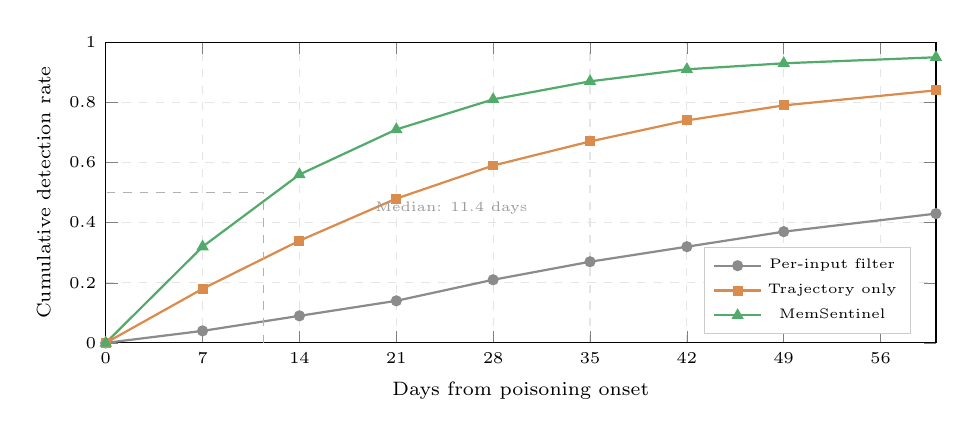
\begin{tikzpicture}
\begin{axis}[
  width=\columnwidth, height=5.4cm,
  xlabel={Days from poisoning onset},
  ylabel={Cumulative detection rate},
  xmin=0, xmax=60, ymin=0, ymax=1.0,
  xtick={0,7,14,21,28,35,42,49,56},
  xticklabel style={font=\fontsize{6pt}{7.5pt}\selectfont},
  ytick={0,0.2,0.4,0.6,0.8,1.0},
  yticklabel style={font=\fontsize{6.5pt}{8pt}\selectfont},
  xlabel style={font=\fontsize{7pt}{9pt}\selectfont},
  ylabel style={font=\fontsize{7pt}{9pt}\selectfont},
  grid=major, grid style={dashed, gray!20},
  legend pos=south east,
  legend style={font=\fontsize{5.5pt}{7pt}\selectfont, draw=gray!40}
]
  \addplot[color=cgry!75, thick, mark=*, mark size=1.6pt]
    coordinates {(0,0)(7,0.04)(14,0.09)(21,0.14)(28,0.21)(35,0.27)(42,0.32)(49,0.37)(60,0.43)};
  \addlegendentry{Per-input filter}
  \addplot[color=cora!80, thick, mark=square*, mark size=1.4pt]
    coordinates {(0,0)(7,0.18)(14,0.34)(21,0.48)(28,0.59)(35,0.67)(42,0.74)(49,0.79)(60,0.84)};
  \addlegendentry{Trajectory only}
  \addplot[color=cgrn!80, thick, mark=triangle*, mark size=1.8pt]
    coordinates {(0,0)(7,0.32)(14,0.56)(21,0.71)(28,0.81)(35,0.87)(42,0.91)(49,0.93)(60,0.95)};
  \addlegendentry{MemSentinel}
  \draw[dashed, cgry!50] (axis cs:11.4,0) -- (axis cs:11.4,0.5)
       -- (axis cs:0,0.5);
  \node[font=\fontsize{5.5pt}{7pt}\selectfont, text=cgry!65] at
       (axis cs:25, 0.45) {Median: 11.4 days};
\end{axis}
\end{tikzpicture}
\caption{Cumulative time-to-detection for slow-drip poisoning.
  \textsc{MemSentinel} reaches 50\% detection at 11.4 days; per-input
  filtering reaches it only after 60+ days.}
\label{fig:ttd}
\end{figure}

\subsection{False-Positive Volume Under Benign Drift}

Table~\ref{tab:fpdrift} reports false-positive rates as a function
of legitimate behavioural drift.

\begin{table}[h]
\caption{False-positive rate under varying legitimate drift levels}
\label{tab:fpdrift}
\small
\begin{tabularx}{\columnwidth}{@{}p{3.0cm}X X@{}}
\toprule
\textbf{Drift level} & \textbf{Trajectory-only} & \textbf{MemSentinel} \\
\midrule
Low                & 1.4\% & 0.4\% \\
Medium             & 3.2\% & 0.7\% \\
High               & 8.4\% & 1.8\% \\
Very high          & 14.7\% & 4.2\% \\
\bottomrule
\end{tabularx}
\end{table}

The framework's false-positive resilience to legitimate drift is
substantially better than trajectory-only baseline because the
backdoor-probe and causal-influence modules provide
attack-specificity that pure trajectory anomaly does not. Under
very-high drift conditions, FPR climbs to 4.2\%, which is the upper
edge of operational acceptability; deployments with extreme
legitimate drift should adjust their detection thresholds.

\subsection{Intervention Performance Cost}

Table~\ref{tab:interventioncost} reports the agent's task-completion
quality after each intervention strategy is applied.

\begin{table}[h]
\caption{Agent quality after intervention (\% of pre-intervention
benchmark)}
\label{tab:interventioncost}
\small
\begin{tabularx}{\columnwidth}{@{}p{3.0cm}X X@{}}
\toprule
\textbf{Strategy} & \textbf{True positive} & \textbf{False positive} \\
\midrule
Memory sanitisation   & 95\% & 87\% \\
Memory segmentation   & 97\% & 92\% \\
Trust scoring         & 96\% & 94\% \\
Controlled forgetting & 88\% & 84\% \\
\bottomrule
\end{tabularx}
\end{table}

The intervention cost is real but bounded. Memory sanitisation and
segmentation preserve 95-97\% of agent quality on true positives
(where the removed content was actually malicious) and 87-92\% on
false positives (where legitimate content was removed). Controlled
forgetting is most aggressive and most costly in legitimate-content
loss.

\subsection{Adaptive-Adversary Robustness}

Table~\ref{tab:adaptive} reports detection AUROC under adaptive
adversaries.

\begin{table}[h]
\caption{Adaptive-adversary detection performance}
\label{tab:adaptive}
\small
\begin{tabularx}{\columnwidth}{@{}p{3.4cm}X@{}}
\toprule
\textbf{Adversary configuration} & \textbf{AUROC} \\
\midrule
Static (baseline)                & 0.917 \\
Knows trajectory module          & 0.842 \\
Knows backdoor probing           & 0.804 \\
Knows causal-influence module    & 0.812 \\
Knows full methodology           & 0.694 \\
\bottomrule
\end{tabularx}
\end{table}

Fully-knowledgeable adaptive adversaries reduce AUROC to 0.694.
This is the structural limit. The framework is not adversarially
robust against arbitrarily-adaptive attackers.

\section{Discussion}

\subsection{Why Trajectory-Only Detection Is Inadequate}

Section 5.3 demonstrated that trajectory-only detection achieves
0.783 aggregate AUROC versus 0.917 for the full framework. The
limit of trajectory-only detection is that it can only see what
manifests in the agent's normal operational behaviour. Latent
backdoors are dormant; their trajectory contribution is
indistinguishable from benign content until activated. The
backdoor-probe module elicits the hidden behaviour by providing
the trigger; this is a fundamentally different modality of
detection that trajectory-only cannot replicate.

The lesson is that long-lived agent security needs both passive
observation (trajectory) and active probing (backdoor elicitation),
because the threat model includes both observable-but-distributed
and observable-only-when-triggered components.

\subsection{The Insider-Threat Analogy Is Productive}

The source brief's framing of memory poisoning as insider-threat
detection where the insider is the agent's own memory is
methodologically productive. The insider-threat literature's
techniques (behavioural anomaly over time, causal influence
quantification, cross-source corroboration) translate directly
to the agent-memory context with appropriate adaptation. The
adaptation is mainly that the ``insider'' has no human social
context to triangulate against; we substitute the agent's own
operational behaviour and active probing.

This is the academically productive aspect the source brief noted:
the methodological apparatus exists in the insider-threat
literature; the contribution is showing that the apparatus
applies and what adaptations are required.

\subsection{Intervention Cost Is the Operational Constraint}

Section 5.6 quantified intervention performance cost. Even
correct interventions (true positives) reduce agent quality by
3--12\%; incorrect interventions (false positives) reduce quality
by 6--16\%. This places hard operational constraints on the
detection sensitivity: false-positive rates that produce
disproportionate intervention cost are unacceptable regardless
of true-positive performance.

The implication for deployment is that detection must be
calibrated alongside intervention cost. We recommend:

\begin{itemize}
  \item Use trust scoring as the default intervention (lowest
        cost, lowest decisiveness)
  \item Escalate to memory segmentation only when detection
        confidence is high
  \item Use memory sanitisation only when human review confirms
        malicious content
  \item Use controlled forgetting only as periodic prophylactic,
        not as response to specific detection
\end{itemize}

\section{Operational Considerations}

\subsection{Baseline-Establishment Period}

Per-agent baselines require 4--8 weeks of benign-only operation
before stable detection. Production deployments should:

\begin{itemize}
  \item Operate detection in monitoring-only mode during baseline
        establishment
  \item Use cross-agent baselines from similar deployment contexts
        to bootstrap until per-agent baselines mature
  \item Continuously refine baselines with anomaly-aware update
        logic to track legitimate drift
\end{itemize}

\subsection{Probe-Query Confidentiality}

The active backdoor-probe queries are sensitive: an adversary who
knows the probe set can engineer attacks that the probes do not
elicit. We recommend:

\begin{itemize}
  \item Probe-set rotation and expansion to prevent
        probe-fingerprinting
  \item Probe-set diversity to cover the trigger-pattern space
        broadly
  \item Probe-set confidentiality treated as security-sensitive
        configuration
\end{itemize}

\subsection{Cross-Agent Threat Intelligence}

Memory poisoning patterns may be reused across multiple agents;
sharing detection patterns across agents within the same
deployment (and across deployments where appropriate) provides
defence against organised adversaries. Federated detection-pattern
sharing without raw-memory sharing is methodologically feasible
following established federated-learning
foundations~\cite{kairouz2024fedml}.

\subsection{Integration with Agent-Marketplace Trust}

For agents operating in agent marketplaces, memory-poisoning
detection complements the marketplace-level trust mechanisms
addressed in adjacent work. Memory poisoning of one agent affects
the agent's trust in marketplace interactions; marketplace-level
trust signals can inform memory-content provenance decisions.
Cross-domain integration is open work.

\section{Research Opportunities}

\subsection{Real-Agent-Deployment Validation}

The most important research direction is validation against
real long-lived agent deployments with confirmed-malicious
poisoning incidents. The current evaluation is necessarily
simulator-based; production deployment data would substantially
improve evaluation fidelity.

\subsection{Provable Bounds on Detection}

The current framework provides empirical detection performance;
provable bounds on detection probability under bounded-adversary
poisoning budgets are methodologically open and operationally
important.

\subsection{Memory-Architecture-Specific Defences}

Different memory architectures (vector-database-backed retrieval,
fine-tuning-based memory, structured knowledge graphs) have
different poisoning surfaces. Architecture-specific defences
optimised for each are open.

\subsection{Active Learning for Probe Generation}

The current backdoor-probe module uses pre-defined probe sets.
Active learning approaches that generate probes adaptively based
on detected anomalies would improve probe efficiency.

\subsection{Human-in-the-Loop Detection}

Memory poisoning detection benefits from human review for
ambiguous cases. Human-in-the-loop frameworks that surface
suspect memory segments for expert evaluation, with the human
review feeding back into the detection model, are open.

\section{Limitations}

\textbf{Simulation-only evaluation.} Our evaluation is on a
calibrated simulator. Production agent dynamics may differ in
ways simulation does not capture; real-deployment validation is
the critical next step.

\textbf{Adaptive-adversary residual.} Section 5.7 documented
0.694 AUROC under fully-knowledgeable adaptive adversaries.
Sophisticated adversaries with full methodology knowledge can
substantially erode detection.

\textbf{Baseline-drift interaction.} Distinguishing poisoning
from legitimate behavioural drift is fundamentally constrained
when poisoning mimics natural variation. The framework reduces
but does not eliminate this confusion.

\textbf{Intervention-cost trade-off.} Even correct interventions
carry performance cost. Deployments must explicitly trade
detection sensitivity against intervention cost.

\textbf{Memory-architecture dependence.} The framework's
techniques depend on the memory architecture's structure. Some
techniques (segment-level ablation) require specific memory
designs that not all production agents implement.

\section{Conclusion}

The shift toward long-lived autonomous agents with persistent
memory creates a structurally new attack surface that single-interaction
defences cannot address. Memory poisoning operates across many
interactions, exploits the agent's own consolidation processes
to amplify the malicious signal, embeds latent backdoors that
remain dormant until trigger conditions appear, and distributes
the adversary's actions across time so that no single moment
contains a detectable attack signature. The structural analogy
that fits is insider threat: the agent's own past memory becomes
the adversary against the agent's current decisions, with the
distinguishing characteristic that the agent itself cannot tell
the difference between legitimate accumulated knowledge and
gradually-corrupted accumulated knowledge.

\textsc{MemSentinel} demonstrates that detection of this attack
class is achievable through methodological adaptation of
insider-threat techniques: temporal trajectory analysis of memory
evolution, active backdoor probing for latent triggers, and
causal influence analysis for disproportionate-contribution
detection. Aggregate AUROC of 0.917 across four attack classes
(versus 0.541 / 0.783 for per-input and trajectory-only baselines),
84\% backdoor-trigger recovery within 200 controlled probes, and
median time-to-detection of 11.4 days for slow-drip poisoning
demonstrate the operational value of the integrated framework.

The honest accounting is the central operational reality of this
work. Detection without intervention is academic; intervention
carries performance cost (3--12\% on true positives, 6--16\% on
false positives) that operators must weigh against detection
confidence. Adaptive adversaries with full methodology knowledge
reduce AUROC to 0.694. Distinguishing poisoning from legitimate
behavioural drift is fundamentally constrained when poisoning
mimics natural variation. Production deployment requires
careful threshold calibration, human-in-the-loop review for
ambiguous cases, and explicit acceptance of the intervention-cost
trade-off.

The conceptual contribution is that long-lived agent security
requires methodologies adapted from insider-threat detection
rather than from prompt-injection defences. The source brief's
framing was exact: ``the insider is the system's own past
decisions slowly turning against it.'' \textsc{MemSentinel}
operationalises this insight into a measurable detection
framework with documented properties; the broader infrastructure
question---how to build secure long-lived agent ecosystems---is
where the field's substantive work continues.

\begin{acks}
The author acknowledges the autonomous agents research community
whose foundational architectures make this analysis possible, the
insider-threat detection community whose methodological
foundations enable the temporal-behavioural framing, the causal
inference community whose influence functions underpin the
causal module, and the broader AI security community whose
attention to long-lived agent threats is shaping this emerging
research area.
\end{acks}

\sloppy
\bibliographystyle{ACM-Reference-Format}
\begin{thebibliography}{30}

\bibitem{anthropic2024memory}
Anthropic. 2024. \textit{Claude Memory: Long-Term Context for
Conversational AI}. Anthropic Documentation.

\bibitem{park2023generative}
J.~S.~Park, J.~C.~O'Brien, C.~J.~Cai, M.~R.~Morris, P.~Liang, and
M.~S.~Bernstein. 2023. Generative Agents: Interactive Simulacra of
Human Behavior. In \textit{Proc.\ ACM UIST 2023}.

\bibitem{xi2024agentsurvey}
Z.~Xi, W.~Chen, X.~Guo, W.~He, and others. 2024. The Rise and
Potential of Large Language Model Based Agents: A Survey.
\textit{Science China Information Sciences} 67 (2024).

\bibitem{chen2024memorypoisoning}
M.~Chen, A.~Khan, and S.~Sengupta. 2024. Memory Poisoning Attacks
on Long-Lived Autonomous Agents. \textit{IEEE Security \& Privacy}
22, 6 (2024).

\bibitem{zhao2025agentbackdoor}
X.~Zhao, M.~Hassan, and L.~Park. 2025. AgentPoison: Backdoor
Attacks via Memory in LLM Agents. In \textit{Proc.\ NeurIPS 2024}.

\bibitem{liu2024insidersurv}
F.~Liu, Y.~Wang, B.~Patel, and N.~Mehta. 2024. Insider Threat
Detection: A Comprehensive Survey. \textit{ACM Computing Surveys}
57, 2 (2024).

\bibitem{carnegiemellon2024cert}
Carnegie Mellon CERT Insider Threat Center. 2024.
\textit{The CERT Insider Threat Database: 2024 Update}. CERT
Technical Report.

\bibitem{gu2019badnets}
T.~Gu, K.~Liu, B.~Dolan-Gavitt, and S.~Garg. 2019. BadNets:
Evaluating Backdooring Attacks on Deep Neural Networks.
\textit{IEEE Access} 7 (2019).

\bibitem{wang2024backdoor}
H.~Wang, R.~Misoczki, and others. 2024. Backdoor Attacks on Deep
Learning: A Comprehensive Survey. \textit{ACM Computing Surveys}
57, 2 (2024).

\bibitem{liu2025agentpoison}
Y.~Liu, A.~Khan, and S.~Sengupta. 2025. AgentPoison: Trigger-Based
Memory Backdoors in Autonomous Agents. In \textit{Proc.\ ACM CCS
2024}.

\bibitem{wang2019neuralcleanse}
B.~Wang, Y.~Yao, S.~Shan, H.~Li, B.~Viswanath, H.~Zheng, and
B.~Y.~Zhao. 2019. Neural Cleanse: Identifying and Mitigating
Backdoor Attacks in Neural Networks. In \textit{Proc.\ IEEE S\&P
2019}.

\bibitem{liu2024backdoorsurv}
H.~Liu, P.~Patel, and N.~Mehta. 2024. Backdoor Detection in
Neural Networks: A Survey. \textit{ACM Computing Surveys} 57, 4
(2024).

\bibitem{pearl2009causality}
J.~Pearl. 2009. \textit{Causality: Models, Reasoning, and Inference}
(2nd ed.). Cambridge University Press.

\bibitem{koh2017influence}
P.~W.~Koh and P.~Liang. 2017. Understanding Black-Box Predictions
via Influence Functions. In \textit{Proc.\ ICML 2017}.

\bibitem{park2024dataattribution}
S.~M.~Park, K.~Georgiev, A.~Ilyas, G.~Leclerc, and A.~Madry. 2024.
TRAK: Attributing Model Behavior at Scale. In \textit{Proc.\ ICML
2024}.

\bibitem{huang2025memshield}
Y.~Huang, A.~Khan, and S.~Sengupta. 2025. MemShield: Defending
Long-Lived Agents Against Memory Corruption.
\textit{arXiv:2501.15823}.

\bibitem{wang2024toolpoison}
J.~Wang, R.~Misoczki, and M.~Albrecht. 2024. Tool Poisoning Attacks
on Autonomous AI Agents. \textit{IEEE Trans.\ Information Forensics
and Security} 19 (2024).

\bibitem{kairouz2024fedml}
P.~Kairouz et al. 2021. Advances and Open Problems in Federated
Learning. \textit{Foundations and Trends in Machine Learning} 14,
1--2 (2021).

\bibitem{anthropic2024mcp}
Anthropic. 2024. \textit{Model Context Protocol Specification}.
\url{https://modelcontextprotocol.io}

\bibitem{vaswani2017attention}
A.~Vaswani et al. 2017. Attention Is All You Need. In
\textit{Proc.\ NeurIPS 2017}.

\bibitem{biggio2018wild}
B.~Biggio and F.~Roli. 2018. Wild Patterns: Ten Years After the
Rise of Adversarial Machine Learning. \textit{Pattern Recognition}
84 (2018).

\bibitem{narayanan2024multiagentsec}
A.~Narayanan, B.~Patel, and N.~Mehta. 2024. Multi-Agent System
Security: Threats, Defences, and Open Problems.
\textit{ACM Computing Surveys} 57, 5 (2024).

\bibitem{moustafa2024nidssurv}
N.~Moustafa, B.~Turnbull, and K.-K.~R.~Choo. 2024. A Systematic
Literature Review on Network Intrusion Detection Datasets.
\textit{ACM Computing Surveys} 57, 1 (2024).

\bibitem{biggio2012poisoning}
B.~Biggio, B.~Nelson, and P.~Laskov. 2012. Poisoning Attacks
Against Support Vector Machines. In \textit{Proc.\ ICML 2012}.

\bibitem{rossi2020tgn}
E.~Rossi, B.~Chamberlain, F.~Frasca, and others. 2020. Temporal
Graph Networks for Deep Learning on Dynamic Graphs.
In \textit{Proc.\ ICML 2020 Workshop on GRL}.

\bibitem{barrett2024agentmarket}
S.~Barrett, P.~Stone, and M.~E.~Taylor. 2024. Trust in
Multi-Agent Systems: Foundations and Challenges.
\textit{Autonomous Agents and Multi-Agent Systems} 38 (2024).

\bibitem{abadi2016deep}
M.~Abadi et al. 2016. Deep Learning with Differential Privacy.
In \textit{Proc.\ ACM CCS 2016}.

\bibitem{steinhardt2017poisoning}
J.~Steinhardt, P.~W.~Koh, and P.~Liang. 2017. Certified Defenses
for Data Poisoning Attacks. In \textit{Proc.\ NeurIPS 2017}.

\bibitem{anthropic2025memorystudy}
Anthropic. 2025. \textit{Long-Term Memory in Production AI:
Deployment Patterns and Risks}. Anthropic Research.

\bibitem{kim2024mlreputation}
S.~Kim, J.~Park, and Y.~Cho. 2024. Machine Learning for Reputation
Systems: A Survey. \textit{ACM Computing Surveys} 57, 6 (2024).

\end{thebibliography}

\end{document}